%  LaTeX support: latex@mdpi.com
%  For support, please attach all files needed for compiling as well as the log file, and specify your operating system, LaTeX version, and LaTeX editor.

%=================================================================
% pandoc conditionals added to preserve backwards compatibility with previous versions of rticles

\documentclass[remotesensing,article,submit,moreauthors,pdftex]{Definitions/mdpi}


%% Some pieces required from the pandoc template
\setlist[itemize]{leftmargin=*,labelsep=5.8mm}
\setlist[enumerate]{leftmargin=*,labelsep=4.9mm}


%--------------------
% Class Options:
%--------------------

%---------
% article
%---------
% The default type of manuscript is "article", but can be replaced by:
% abstract, addendum, article, book, bookreview, briefreport, casereport, comment, commentary, communication, conferenceproceedings, correction, conferencereport, entry, expressionofconcern, extendedabstract, datadescriptor, editorial, essay, erratum, hypothesis, interestingimage, obituary, opinion, projectreport, reply, retraction, review, perspective, protocol, shortnote, studyprotocol, systematicreview, supfile, technicalnote, viewpoint, guidelines, registeredreport, tutorial
% supfile = supplementary materials

%----------
% submit
%----------
% The class option "submit" will be changed to "accept" by the Editorial Office when the paper is accepted. This will only make changes to the frontpage (e.g., the logo of the journal will get visible), the headings, and the copyright information. Also, line numbering will be removed. Journal info and pagination for accepted papers will also be assigned by the Editorial Office.

%------------------
% moreauthors
%------------------
% If there is only one author the class option oneauthor should be used. Otherwise use the class option moreauthors.

%---------
% pdftex
%---------
% The option pdftex is for use with pdfLaTeX. Remove "pdftex" for (1) compiling with LaTeX & dvi2pdf (if eps figures are used) or for (2) compiling with XeLaTeX.

%=================================================================
% MDPI internal commands - do not modify
\firstpage{1}
\makeatletter
\setcounter{page}{\@firstpage}
\makeatother
\pubvolume{1}
\issuenum{1}
\articlenumber{0}
\pubyear{2023}
\copyrightyear{2023}
%\externaleditor{Academic Editor: Firstname Lastname}
\datereceived{ }
\daterevised{ } % Comment out if no revised date
\dateaccepted{ }
\datepublished{ }
%\datecorrected{} % For corrected papers: "Corrected: XXX" date in the original paper.
%\dateretracted{} % For corrected papers: "Retracted: XXX" date in the original paper.
\hreflink{https://doi.org/} % If needed use \linebreak
%\doinum{}
%\pdfoutput=1 % Uncommented for upload to arXiv.org

%=================================================================
% Add packages and commands here. The following packages are loaded in our class file: fontenc, inputenc, calc, indentfirst, fancyhdr, graphicx, epstopdf, lastpage, ifthen, float, amsmath, amssymb, lineno, setspace, enumitem, mathpazo, booktabs, titlesec, etoolbox, tabto, xcolor, colortbl, soul, multirow, microtype, tikz, totcount, changepage, attrib, upgreek, array, tabularx, pbox, ragged2e, tocloft, marginnote, marginfix, enotez, amsthm, natbib, hyperref, cleveref, scrextend, url, geometry, newfloat, caption, draftwatermark, seqsplit
% cleveref: load \crefname definitions after \begin{document}

%=================================================================
% Please use the following mathematics environments: Theorem, Lemma, Corollary, Proposition, Characterization, Property, Problem, Example, ExamplesandDefinitions, Hypothesis, Remark, Definition, Notation, Assumption
%% For proofs, please use the proof environment (the amsthm package is loaded by the MDPI class).

%=================================================================
% Full title of the paper (Capitalized)
\Title{Identifying Heterogeneity in SAR Data with New Test Statistics}

% MDPI internal command: Title for citation in the left column
\TitleCitation{Identifying Heterogeneity in SAR Data with New Test
Statistics}

% Author Orchid ID: enter ID or remove command
%\newcommand{\orcidauthorA}{0000-0000-0000-000X} % Add \orcidA{} behind the author's name
%\newcommand{\orcidauthorB}{0000-0000-0000-000X} % Add \orcidB{} behind the author's name


% Authors, for the paper (add full first names)
\Author{Alejandro C.
Frery$^{1,*}$\href{https://orcid.org/0000-0002-8002-5341}
{\orcidicon}, Janeth
Alpala$^{2}$\href{https://orcid.org/0000-0002-0265-6236}
{\orcidicon}, Abraão D. C.
Nascimento$^{2}$\href{https://orcid.org/0000-0003-2673-219X}
{\orcidicon}}


%\longauthorlist{yes}


% MDPI internal command: Authors, for metadata in PDF
\AuthorNames{Alejandro C. Frery, Janeth Alpala, Abraão D. C. Nascimento}

% MDPI internal command: Authors, for citation in the left column
%\AuthorCitation{Lastname, F.; Lastname, F.; Lastname, F.}
% If this is a Chicago style journal: Lastname, Firstname, Firstname Lastname, and Firstname Lastname.
\AuthorCitation{Frery, A.C.; Alpala, J.; Nascimento,A.D.C.}

% Affiliations / Addresses (Add [1] after \address if there is only one affiliation.)
\address{%
$^{1}$ \quad School of Mathematics and Statistics, Victoria University
of Wellington, Wellington 6140, New Zealand; \\
$^{2}$ \quad Departamento de Estatística, Universidade Federal de
Pernambuco, Recife 50670-901, PE, Brazil; \\
}

% Contact information of the corresponding author
\corres{Correspondence: \href{mailto:alejandro.frery@vuw.ac.nz}{\nolinkurl{alejandro.frery@vuw.ac.nz}}}

% Current address and/or shared authorship








% The commands \thirdnote{} till \eighthnote{} are available for further notes

% Simple summary

%\conference{} % An extended version of a conference paper

% Abstract (Do not insert blank lines, i.e. \\)
\abstract{
This paper presents a statistical approach to identify the underlying roughness properties in synthetic aperture radar (SAR) intensity data. 
The physical modeling of this type of data allows the use of the gamma distribution in the presence of fully developed speckle, i.e. when there are infinitely many independent backscatters per resolution cell. This situation is often referred to as ``homogeneous'' or ``textureless'' regions. 
The \(\mathcal{G}_I^0\) distribution is also a widely accepted law for heterogeneous and extremely heterogeneous regions. 
We propose three test statistics to distinguish between homogeneous and inhomogeneous regions, i.e. between gamma and \(\mathcal{G}_I^0\) distributed data, both with a known number of looks. 
The first test statistic uses a bootstrapped nonparametric estimator of Shannon entropy, which provides a robust assessment in the face of uncertain distributional assumptions.
The second test uses the classical coefficient of variation. 
The third test uses an alternative form of estimating the CV based on the ratio of the mean absolute deviation from the median to the median. 
We apply our test statistic to create maps of \(p\) values for the hypothesis of homogeneity. These maps identify different types of targets. 
We show that our proposal outperforms its competitors using simulated and SAR data.}


% Keywords
\keyword{SAR; heterogeneity; entropy; coefficient of variation;
hypothesis tests}

% The fields PACS, MSC, and JEL may be left empty or commented out if not applicable
%\PACS{J0101}
%\MSC{}
%\JEL{}

%%%%%%%%%%%%%%%%%%%%%%%%%%%%%%%%%%%%%%%%%%
% Only for the journal Diversity
%\LSID{\url{http://}}

%%%%%%%%%%%%%%%%%%%%%%%%%%%%%%%%%%%%%%%%%%
% Only for the journal Applied Sciences

%%%%%%%%%%%%%%%%%%%%%%%%%%%%%%%%%%%%%%%%%%

%%%%%%%%%%%%%%%%%%%%%%%%%%%%%%%%%%%%%%%%%%
% Only for the journal Data



%%%%%%%%%%%%%%%%%%%%%%%%%%%%%%%%%%%%%%%%%%
% Only for the journal Toxins


%%%%%%%%%%%%%%%%%%%%%%%%%%%%%%%%%%%%%%%%%%
% Only for the journal Encyclopedia


%%%%%%%%%%%%%%%%%%%%%%%%%%%%%%%%%%%%%%%%%%
% Only for the journal Advances in Respiratory Medicine
%\addhighlights{yes}
%\renewcommand{\addhighlights}{%

%\noindent This is an obligatory section in “Advances in Respiratory Medicine”, whose goal is to increase the discoverability and readability of the article via search engines and other scholars. Highlights should not be a copy of the abstract, but a simple text allowing the reader to quickly and simplified find out what the article is about and what can be cited from it. Each of these parts should be devoted up to 2~bullet points.\vspace{3pt}\\
%\textbf{What are the main findings?}
% \begin{itemize}[labelsep=2.5mm,topsep=-3pt]
% \item First bullet.
% \item Second bullet.
% \end{itemize}\vspace{3pt}
%\textbf{What is the implication of the main finding?}
% \begin{itemize}[labelsep=2.5mm,topsep=-3pt]
% \item First bullet.
% \item Second bullet.
% \end{itemize}
%}


%%%%%%%%%%%%%%%%%%%%%%%%%%%%%%%%%%%%%%%%%%


% tightlist command for lists without linebreak
\providecommand{\tightlist}{%
  \setlength{\itemsep}{0pt}\setlength{\parskip}{0pt}}



\usepackage[english]{babel}
\usepackage{bm,bbm}
\usepackage{mathrsfs}
\usepackage{siunitx}
\usepackage{graphicx}
\usepackage{url}
\usepackage[T1]{fontenc}
\usepackage{polski}
\usepackage{booktabs}
\usepackage{color}
\usepackage{amsmath}
\usepackage{multirow}
\usepackage{subcaption}
\captionsetup[sub]{labelfont=bf,textfont=bf}
\usepackage{longtable}
\usepackage{booktabs}
\usepackage{array}
\usepackage{multirow}
\usepackage{wrapfig}
\usepackage{float}
\usepackage{colortbl}
\usepackage{pdflscape}
\usepackage{tabu}
\usepackage{threeparttable}
\usepackage{threeparttablex}
\usepackage[normalem]{ulem}
\usepackage{makecell}
\usepackage{xcolor}

\begin{document}



%%%%%%%%%%%%%%%%%%%%%%%%%%%%%%%%%%%%%%%%%%

\setlength{\tabcolsep}{6pt} 
\newcommand{\bias}{\operatorname{Bias}}
\newcommand{\widebar}[1]{\overline{#1}}

\hypertarget{sec:Introduction}{%
\section{Introduction}\label{sec:Introduction}}

Synthetic Aperture Radar (SAR) technology has become an important tool for environmental monitoring and disaster management. It provides valuable images under various conditions, including day or night and different weather situations~\cite{Moreira2013,Mu2019}. However, the effective use of SAR data depends on a thorough understanding of its statistical properties, especially the impact of speckle effects inherent in SAR data due to the coherent nature of the imaging process~\cite{Argenti2013}.

In the presence of non-Gaussian speckle interference, SAR data requires a reliable statistical model for accurate processing. The
\(\mathcal{G}^0\) distribution, which is suitable for SAR data, includes the
Gamma law as the limiting case for fully developed speckle~\cite{Ferreira2020} and provides flexibility with fewer parameters for analysis.

Our work aims to improve the identification of potential roughness features in SAR intensity data. Physical modeling of SAR data allows to take advantage of the gamma distribution in the presence of fully developed speckles and to create a scenario with an infinite number of independent backscatterers per resolution unit, often referred to as homogeneous regions.

In this context, we present a set of three novel test statistics that aim to distinguish between homogeneous and non-homogeneous domains, in particular between gamma and
\(\mathcal{G}^0\) distributed data, each with a known number of looks. To understand the core ideas behind our approach, we explore the use of properties such as entropy and coefficient of variation.

Entropy is a fundamental concept in information theory with far-reaching applications in pattern recognition, statistical physics, stochastic dynamics and statistics. Shannon introduced it in 1948~\cite{Shannon1948} for a random variable as a measure of information and uncertainty.\\
In statistics, Shannon entropy is a crucial descriptive parameter, especially for evaluating data dispersion and performing tests for normality, exponentiality and uniformity~\cite{Wieczorkowski1999,Zamanzade2012}. Entropy estimation is associated with some practical difficulties, especially when the model is unknown. In these cases, non-parametric methods are used.
Spacing methods have been discussed as a non-parametric approach in~\cite{AlizadehNoughabi2010,Subhash2021}. This strategy provides the flexibility to consider a wide range of models without enforcing certain parametric constraints.

The coefficient of variation (CV), introduced in 1896 by Pearson~\cite{Pearson1896}, is a relative dispersion measure widely used in various fields of applied statistics, including sampling, biostatistics, medical and biological research, climatology and other fields
\cite{hendricks1936sampling, Tian2005,SubrahmanyaNairy2003,Chankham2024}.
It facilitates the comparison of variability between different populations and is particularly valuable for comparing variables with different units. This is because when the main purpose is to compare the variations of several variables, the standard deviation can only serve as an adequate measure of variation if all variables are expressed in the same unit of measurement and have identical means. If these conditions are not met for the variables under investigation, the CV is the relative measure that is usually used in real applications. The variable with the highest CV value is the one with the largest relative dispersion around the mean value~\cite{Banik2011}.

In our study, entropy serves as a fundamental parameter that allows a robust evaluation using a bootstrapped nonparametric estimator of the
Shannon entropy.
At the same time, we use the classical CV and an alternative form based on the ratio between the median absolute deviation and the median. 
The CV is known as an efficient and robust index for texture information and measures the homogeneity of the image~\cite{Lopes1990}.
Applying these test statistics to generate maps of \(p\) values facilitates testing the homogeneity hypothesis and reveals different types of targets in the SAR data. 
Through extensive experiments with real and simulated SAR data, we demonstrate the superiority of our proposed method over existing approaches.

The article is structured as follows: Section~\ref{sec:Background}
deals with statistical modeling and entropy estimation for intensity SAR
data. Section~\ref{sec:test} outlines hypothesis tests based on nonparametric entropy estimators and coefficients of variation. In
Section~\ref{sec:Results} we present experimental results. Finally, in
Section~\ref{sec:conclusion} the conclusions are presented.

\hypertarget{sec:Background}{%
\section{Background}\label{sec:Background}}

\hypertarget{statistical-modeling-of-intensity-sar-data}{%
\subsection{Statistical Modeling of Intensity SAR
data}\label{statistical-modeling-of-intensity-sar-data}}

The primary models used for SAR intensity data include the gamma and the
\(\mathcal{G}_I^0\) distributions~\citep{Frery1997}. The first model is suitable for fully developed speckle and is a limiting case of the second model, which is interesting due to its versatility in accurately representing regions with different roughness properties~\citep{Cassetti2022}.
We denote
\(Z \sim \Gamma_{\text{SAR}}(L, \mu)\) and
\(Z \sim G_I^0(\alpha, \gamma, L)\) to indicate that \(Z\) follows the
distributions characterized by the respective probability density
functions (pdfs): 
\begin{align}
    f_Z(z;L, \mu)&=\frac{L^L}{\Gamma(L)\mu^L}z^{L-1}\exp\left\{-Lz/\mu\right\} \mathbbm 1_{\mathbbm R_+}(z)\label{E:gamma1}\\
    \intertext{ and }
    f_Z(z; \alpha, \gamma, L)&=\frac{L^L\Gamma(L-\alpha)}{\gamma^{\alpha}\Gamma(-\alpha)\Gamma(L)}\cdot\frac{z^{L-1}}{(\gamma+Lz)^{L-\alpha}} \mathbbm 1_{\mathbbm R_+}(z),\label{E:gi01}
\end{align} 
where \(\mu > 0\) is the mean, \(\gamma > 0\) is the scale, \(\alpha < -1\) measures
the roughness, \(L \geq 1\) is the number of looks, \(\Gamma(\cdot)\) is
the gamma function, and \(\mathbbm 1_{A}(z)\) is the indicator function
of the set \(A\).

If we take the law with the density~\eqref{E:gi01}, the \(r\)th non-central moment of \(Z\) is expressed as follows:
\begin{align}
    E_{G_I^0}\left(Z^r\right)=\left(\frac{\gamma}{L}\right)^r\frac{\Gamma(-\alpha-r)}{\Gamma(-\alpha)}\cdot\frac{\Gamma(L+r)}{\Gamma(L)}, \quad \alpha <-r. 
    \label{E:rmom}
\end{align}

Although the \(\mathcal{G}_I^0\) distribution is defined by the parameters \(\alpha\) and \(\gamma\), in the SAR literature~\cite{Nascimento2010} the texture \(\alpha\) and the mean \(\mu\) are usually used. In this way, we calculate the expected value \(\mu\) using the expression in~\eqref{E:rmom}, and we reparametrize~\eqref{E:gi01} with \(\mu\),
\(\alpha\), and \(L\).
Then \begin{align*}
    \mu=\left(\frac{\gamma}{L}\right)\frac{\Gamma(-\alpha-1)}{\Gamma(-\alpha)}\cdot\frac{\Gamma(L+1)}{\gamma(L)}=-\frac{\gamma}{\alpha+1}.
\end{align*} 
The reparametrized pdf that characterizes the law \(G_I^0(\mu, \alpha, L)\) is thus
\begin{equation}
        f_Z(z; \mu, \alpha, L)=\frac{L^L\Gamma(L-\alpha)}{\big[-\mu(\alpha+1)\big]^{\alpha}\Gamma(-\alpha)\Gamma(L)} \frac{z^{L-1}}{\big[-\mu(\alpha+1)+Lz\big]^{L-\alpha}}.\label{E:gi02}
\end{equation}

\hypertarget{the-shannon-entropy}{%
\subsection{The Shannon Entropy}\label{the-shannon-entropy}}

The parametric representation of the Shannon entropy for a system described by a continuous random variable is:
\begin{equation}
  \label{E:entropy2}
  H(Z)=-\int_{-\infty }^\infty \ f(z)\ln f(z)\, \mathrm{d}z,
\end{equation} 
here, \(f(\cdot)\) is the pdf
that characterizes the distribution of the real-valued random variable
\(Z\).

Using~\eqref{E:entropy2}, we can express the Shannon entropy of
\(\Gamma_{\text{SAR}}\)in~\eqref{E:gamma1} and \(G_I^0\)
in~\eqref{E:gi02} based on~\cite{Cassetti2022} and~\cite{Ferreira2020}:
\begin{equation}
\label{E:E-gamma}
H_{\Gamma_{\text{SAR}}}(L, \mu) =   L -\ln L+\ln\Gamma(L)+(1-L)\psi^{(0)}(L) + \ln \mu, 
\end{equation} \begin{multline}
\label{E:E-GIO}
H_{G_I^0}(\mu, \alpha, L) =L -\ln L+\ln\Gamma(L)+(1-L)\psi^{(0)}(L) +\ln \mu -\ln\Gamma(L-\alpha)\\
+ (L-\alpha) \psi^{(0)}(L-\alpha)-(1-\alpha)\psi^{(0)}(-\alpha)+\ln (-1-\alpha)+\ln\Gamma(-\alpha)-L,
\end{multline} where \(\psi^{(0)}(\cdot)\) is the digamma function.
Figure~\ref{fig:Plot_GI0_to_gamma1}, shows the behavior of the entropy of \(G_I^0\) when
\(\alpha \in \left\{-\infty, -20, -8, -3\right\}\), where the approximation to the entropy of \(\Gamma_{\text{SAR}}\) can be observed when \(\alpha\)
assumes large negative values.
In an interpretative sense, we can conclude that the more heterogeneous (high values of $\alpha$) the SAR region is, the higher the value of entropy (or degree of disorder).
It is worth noting that this conclusion confirms what is written in the SAR literature.


\begin{figure}[hbt]
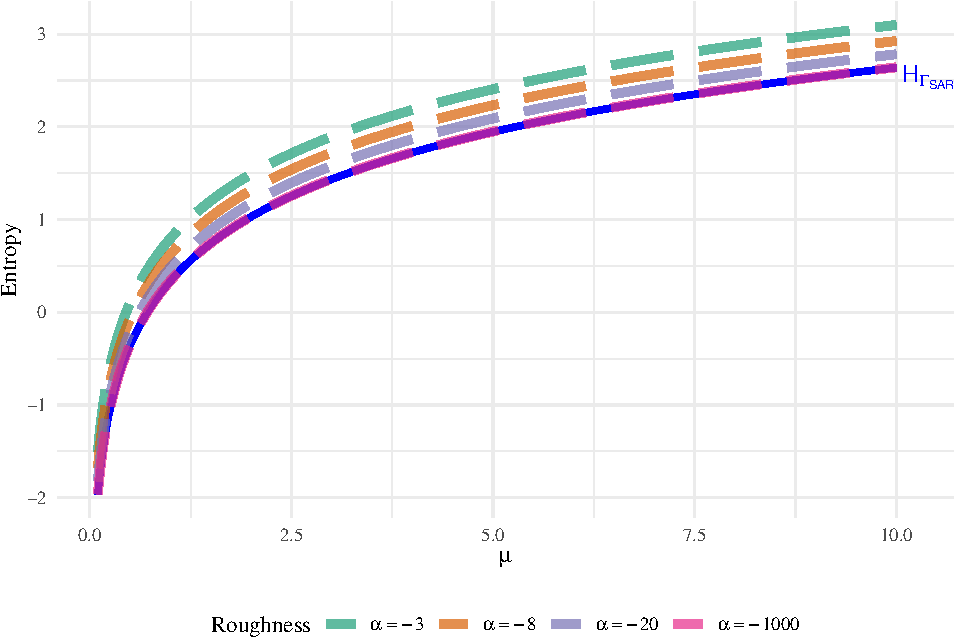
\includegraphics[width=0.7\linewidth]{Identifying-Heterogeneity-in-SAR-Data-with-New-Test-Statistics_files/figure-latex/Plot_GI0_to_gamma1-1} \caption{$H_{ G_I^0}$ converges to the $H_{\Gamma_{\text{SAR}}}$ with $L=8$.}\label{fig:Plot_GI0_to_gamma1}
\end{figure}

\hypertarget{estimation-of-the-shannon-entropy}{%
\subsection{Estimation of the Shannon
Entropy}\label{estimation-of-the-shannon-entropy}}

The problem of non-parametric estimation of \(H(Z)\) has been considered by many authors, including~\cite{vasicek1976test, Wieczorkowski1999,correa1995new,AlOmari2019},
who have proposed estimators based on spacings.

One of the first non-parametric estimators based on spacings was introduced by Vasicek~\cite{vasicek1976test}. Under the assumption that
\(\bm{Z}=(Z_1, Z_2,\ldots,Z_n)\) is a random sample from the distribution \(F(z)\), the estimator is defined as:
\begin{equation*}
\label{E:Vas}
    \widehat{H}_{\text{V}}(\bm{Z})=\frac{1}{n}\sum_{i=1}^{n}\ln\left[\frac{n}{2m}\left(Z_{(i+m)}-Z_{(i-m)}\right)\right],
    \end{equation*} where \(m<n/2\) is a positive integer,
\(Z_{(i+m)}-Z_{(i-m)}\) is the \(m\)-spacing and
\(Z_{(1)}\leq Z_{(2)}\leq\ldots\leq Z_{(n)}\) are the order statistics
and \(Z_{(i)}= Z_{(1)}\) if \(i<1\), \(Z_{(i)}= Z_{(n)}\) if \(i>n\).

Several authors have explored adaptations to Vasicek's estimator. 
We consider three estimators known for their superior performance~\cite{Cassetti2022}:
Correa~\cite{correa1995new}, \(\widehat{H}_{\text{C}}\);
Ebrahimi et al~\cite{Ebrahimi1994}, \(\widehat{H}_{\mathrm{E}}\);
and Al Omary~\cite{IbrahimAlOmari2014}, \(\widehat{H}_{\mathrm{AO}}\).

\hypertarget{enhanced-bootstrap-technique}{%
\subsection{Enhanced Bootstrap
Technique}\label{enhanced-bootstrap-technique}}

We use the bootstrap technique to refine the accuracy of existing nonparametric entropy estimators. In this approach, new data sets are generated by replicate sampling from an existing data set~\cite{Michelucci2021}.

Let us assume that non-parametric entropy estimators
\(\widehat{H}=\widehat{\theta}(\bm{Z})\) are inherently biased, i.e:\begin{equation}
\label{Eq:bias1}
\operatorname{Bias}\big(\widehat{\theta}(\bm{Z})\big) = E\big[\widehat{\theta}(\bm{Z})\big] - \theta \neq 0.
\end{equation} Our bootstrap-improved estimators are of the form:
\begin{align*}
\widetilde{H} &= 2\widehat{\theta}(\bm{Z}) - \frac{1}{B}\sum_{b=1}^B \widehat{\theta}_b(\bm{Z}^{(b)}),
\end{align*} 
where \(B\) is the number of replications in the bootstrap
technique. 
Applying this methodology, the original estimators of Correa,
Ebrahimi and Al-Omari are now referred to as the proposed bootstrap-enhanced versions:
\(\widetilde{H}_{\text{C}}\),
\(\widetilde{H}_{\text{E}}\), and \(\widetilde{H}_{\text{AO}}\),
respectively.

We analyzed the performance of these estimators with a Monte Carlo study: \(500\) samples of \(G_I^0\) of size
\(n\in\left\{9, 25, 49, 81, 121\right\}\) and different values for mean, number of looks and roughness. We present the results with
\(\mu\in\left\{1, 10\right\}\), \(\alpha=-10\) and \(L=5\). The results are also adherent for the other situations. In the bootstrap technique, each sample is replicated a hundred times with replacement. We use the following heuristic formula for spacing,
\(m=\left[\sqrt{n}+0.5\right]\).

In Figure~\ref{fig:Plot_bias_mse_gi0} we show comparisons of bias and mean squared error (MSE) between the original non-parametric entropy estimators and their respective bootstrap-enhanced versions. The use of the bootstrap technique shows higher precision, lower bias and MSE, and improved convergence. The results of the simulation can be found in
Table~\ref{tab:table2}.

The precision of the estimators resulting from the comparison of bias and MSE benefits significantly from the bootstrap technique, especially for sample sizes below 81.

\begin{figure}[hbt]
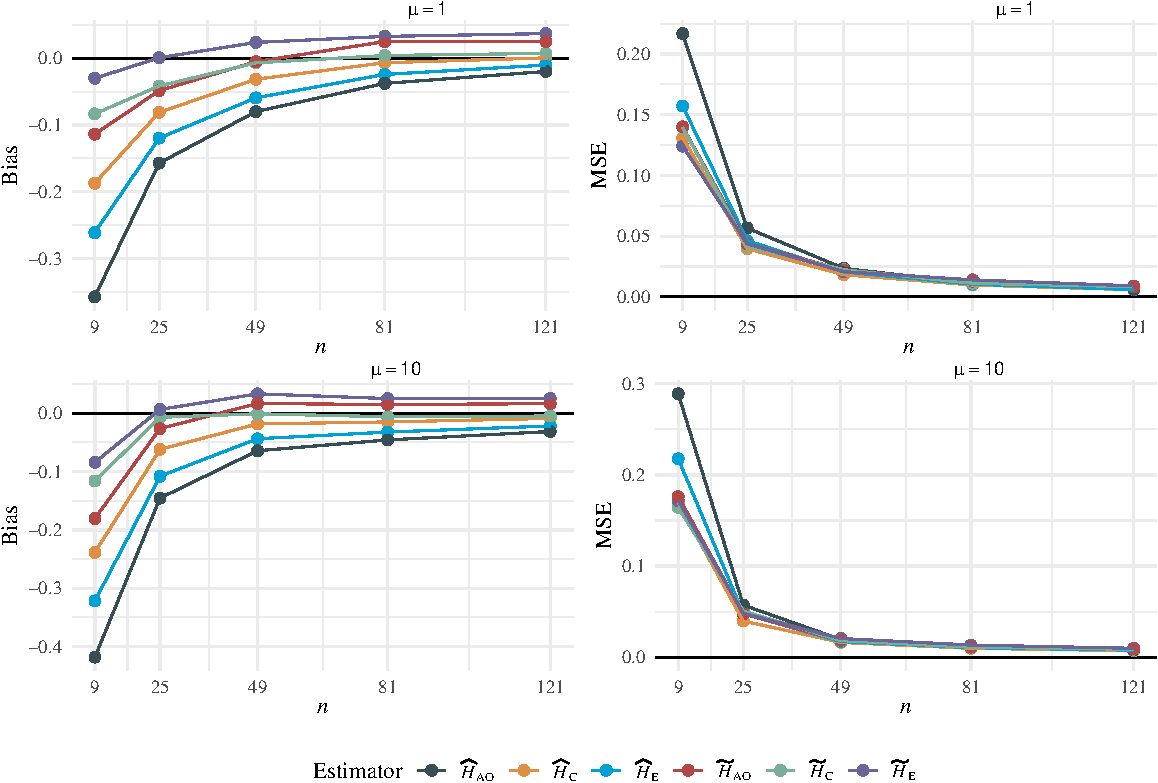
\includegraphics[width=0.8\linewidth]{Identifying-Heterogeneity-in-SAR-Data-with-New-Test-Statistics_files/figure-latex/Plot_bias_mse_gi0-1} \caption{Bias and MSE, $L=5$ and  $\alpha=-10$.}\label{fig:Plot_bias_mse_gi0}
\end{figure}

\begin{table}[H]
\centering
\caption{\label{tab:table2}Bias and MSE of non-parametric entropy estimators and bootstrap versions.}
\resizebox{\ifdim\width>\linewidth\linewidth\else\width\fi}{!}{
\begin{tabular}[t]{lrrrrrrrrrrrrr}
\toprule
\multicolumn{1}{c}{ } & \multicolumn{1}{c}{ } & \multicolumn{6}{c}{Bias} & \multicolumn{6}{c}{MSE} \\
\cmidrule(l{3pt}r{3pt}){3-8} \cmidrule(l{3pt}r{3pt}){9-14}
\multicolumn{1}{c}{$\mu$} & \multicolumn{1}{c}{$n$} & \multicolumn{1}{c}{$\widehat{H}_{\text{AO}}$} & \multicolumn{1}{c}{$\widehat{H}_{\text{C}}$} & \multicolumn{1}{c}{$\widehat{H}_{\text{E}}$} & \multicolumn{1}{c}{$\widetilde{H}_{\text{AO}}$} & \multicolumn{1}{c}{$\widetilde{H}_{\text{C}}$} & \multicolumn{1}{c}{$\widetilde{H}_{\text{E}}$} & \multicolumn{1}{c}{$\widehat{H}_{\text{AO}}$} & \multicolumn{1}{c}{$\widehat{H}_{\text{C}}$} & \multicolumn{1}{c}{$\widehat{H}_{\text{E}}$} & \multicolumn{1}{c}{$\widetilde{H}_{\text{AO}}$} & \multicolumn{1}{c}{$\widetilde{H}_{\text{C}}$} & \multicolumn{1}{c}{$\widetilde{H}_{\text{E}}$}\\
\midrule
 & $9$ & $-0.188$ & $-0.261$ & $-0.358$ & $-0.083$ & $-0.030$ & $-0.114$ & $\phantom{-}0.131$ & $\phantom{-}0.157$ & $\phantom{-}0.217$ & $\phantom{-}0.140$ & $\phantom{-}0.124$ & $\phantom{-}0.140$\\

 & $25$ & $-0.081$ & $-0.120$ & $-0.157$ & $-0.042$ & $\phantom{-}0.001$ & $-0.049$ & $\phantom{-}0.040$ & $\phantom{-}0.046$ & $\phantom{-}0.057$ & $\phantom{-}0.042$ & $\phantom{-}0.044$ & $\phantom{-}0.044$\\

 & $49$ & $-0.032$ & $-0.059$ & $-0.080$ & $-0.007$ & $\phantom{-}0.024$ & $-0.005$ & $\phantom{-}0.018$ & $\phantom{-}0.021$ & $\phantom{-}0.023$ & $\phantom{-}0.022$ & $\phantom{-}0.021$ & $\phantom{-}0.022$\\

 & $81$ & $-0.007$ & $-0.024$ & $-0.038$ & $\phantom{-}0.004$ & $\phantom{-}0.033$ & $\phantom{-}0.025$ & $\phantom{-}0.010$ & $\phantom{-}0.010$ & $\phantom{-}0.011$ & $\phantom{-}0.011$ & $\phantom{-}0.014$ & $\phantom{-}0.013$\\

\multirow{-5}{*}[2\dimexpr\aboverulesep+\belowrulesep+\cmidrulewidth]{\raggedright\arraybackslash 1} & $121$ & $\phantom{-}0.000$ & $-0.010$ & $-0.020$ & $\phantom{-}0.007$ & $\phantom{-}0.037$ & $\phantom{-}0.025$ & $\phantom{-}0.006$ & $\phantom{-}0.006$ & $\phantom{-}0.006$ & $\phantom{-}0.008$ & $\phantom{-}0.009$ & $\phantom{-}0.008$\\
\cmidrule{1-14}
 & $9$ & $-0.239$ & $-0.322$ & $-0.418$ & $-0.116$ & $-0.084$ & $-0.180$ & $\phantom{-}0.169$ & $\phantom{-}0.218$ & $\phantom{-}0.289$ & $\phantom{-}0.164$ & $\phantom{-}0.172$ & $\phantom{-}0.176$\\

 & $25$ & $-0.062$ & $-0.108$ & $-0.145$ & $-0.007$ & $\phantom{-}0.006$ & $-0.026$ & $\phantom{-}0.040$ & $\phantom{-}0.048$ & $\phantom{-}0.057$ & $\phantom{-}0.051$ & $\phantom{-}0.048$ & $\phantom{-}0.047$\\

 & $49$ & $-0.018$ & $-0.044$ & $-0.064$ & $-0.001$ & $\phantom{-}0.033$ & $\phantom{-}0.017$ & $\phantom{-}0.016$ & $\phantom{-}0.017$ & $\phantom{-}0.019$ & $\phantom{-}0.018$ & $\phantom{-}0.020$ & $\phantom{-}0.018$\\

 & $81$ & $-0.015$ & $-0.032$ & $-0.046$ & $-0.006$ & $\phantom{-}0.025$ & $\phantom{-}0.015$ & $\phantom{-}0.010$ & $\phantom{-}0.010$ & $\phantom{-}0.011$ & $\phantom{-}0.011$ & $\phantom{-}0.013$ & $\phantom{-}0.011$\\

\multirow{-5}{*}[2\dimexpr\aboverulesep+\belowrulesep+\cmidrulewidth]{\raggedright\arraybackslash 10} & $121$ & $-0.009$ & $-0.022$ & $-0.031$ & $-0.005$ & $\phantom{-}0.025$ & $\phantom{-}0.016$ & $\phantom{-}0.007$ & $\phantom{-}0.008$ & $\phantom{-}0.008$ & $\phantom{-}0.009$ & $\phantom{-}0.010$ & $\phantom{-}0.009$\\
\bottomrule
\end{tabular}}
\end{table}

\hypertarget{coefficient-of-variation-and-a-robust-alternative}{%
\subsection{Coefficient of variation and a robust
alternative}\label{coefficient-of-variation-and-a-robust-alternative}}

The population CV is defined as the ratio of the population standard deviation \((\sigma)\) to the population mean \((\mu)\):

\begin{align}
    \text{CV}=\frac{\sigma}{\mu}, \quad \text{ for }\mu \neq 0.
\end{align}

We explore a robust alternative to CV, as described in
\cite{Ospina2019}, which incorporates the ratio between the mean absolute deviation from the median (MnAD) and the median, two well-known robust measures of
scale and location, respectively. The sample version for the MnAD is defined as
\(n^{-1}\sum_{i=1}^n|x_i-\widehat{Q}_2|\), where \(\widehat{Q}_2\)
is an estimate for the median of the population, which can be approximated by the median of the sample.

\hypertarget{sec:test}{%
\section{Hypothesis Testing}\label{sec:test}}

We aim at testing the following hypotheses:
\[
 \begin{cases}\mathcal{H}_0: \text{ The data comes from the } \Gamma_{\text{SAR}}\\ 
  \mathcal{H}_1:\text{ The data comes from the } G_I^0.\end{cases}
\] 
In the physical sense, we are testing the hypothesis that the data are fully developed speckle.
As for the parametric problem, once it is not possible to define the hypothesis $\mathcal{H}_0=\alpha=-\infty$, it is impossible to solve this problem with the parametric statistical inference alternatives (such as likelihood ratio, score, grandient and Wald hypothesis test).
The proposed tests to solve this physical problem in SAR systems are described below.

\hypertarget{the-proposed-test-based-on-non-parametric-entropy}{%
\subsection{The Proposed Test Based on Non-parametric
Entropy}\label{the-proposed-test-based-on-non-parametric-entropy}}

The first test statistic evaluates the behavior of the data under the null hypothesis using the empirical distribution: 
\begin{equation}\label{Eq:test_e}
S_H= \widetilde{H}-\left[H_{\Gamma_{\text{SAR}}}(L)+\ln \overline{Z}\right].
\end{equation} 
The values should be zero under the null hypothesis and otherwise far from it.

Figure~\ref{fig:Plot_density} shows the empirical test statistic densities for different sample sizes, and Table~\ref{tab:table_stat_combined}
summarizes the main descriptive statistics, including mean, SD, variance (Var), skewness
(SK), excessive kurtosis (EK) and Anderson--Darling \(p\) values for normality. Results with \(p\) values greater than \(0.05\) do not indicate a violation of the normality assumption. A low variance as well as a skewness and an excessive kurtosis of almost zero indicate limited dispersion, symmetry and a slight tail.\\
Normal QQ plots confirm that there is no evidence against a normal distribution.

\begin{figure}[hbt]
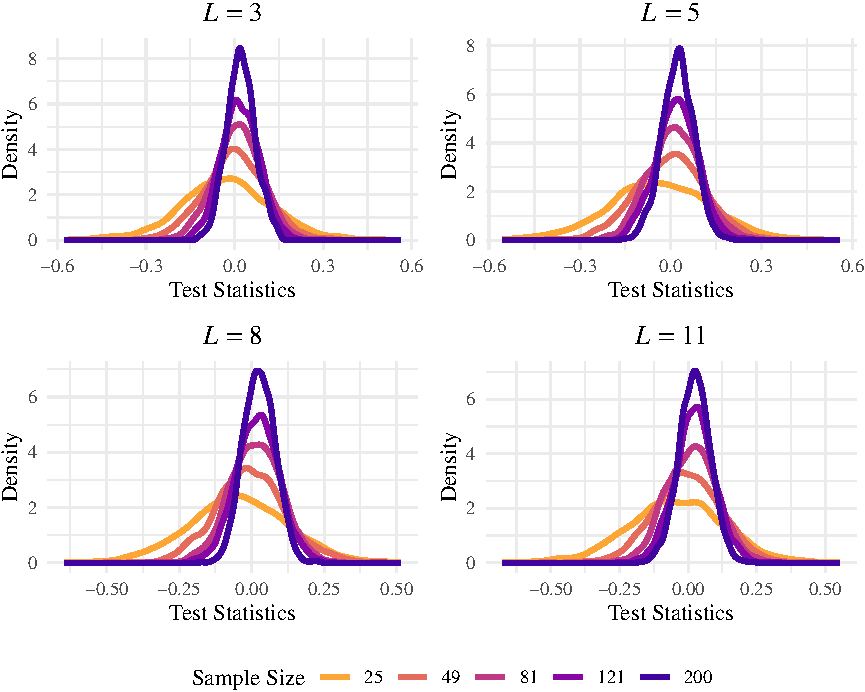
\includegraphics[width=0.8\linewidth]{Identifying-Heterogeneity-in-SAR-Data-with-New-Test-Statistics_files/figure-latex/Plot_density-1} \caption{Empirical density  under the null hypothesis.}\label{fig:Plot_density}
\end{figure}

\begin{table}[H]

\caption{\label{tab:table_stat_combined}Descriptive analysis of $S_H$ with $L\in\left\{3,5, 8,11\right\}$ and $\mu=1$.}
\begin{tabular}[t]{lrrrrrrr}
\toprule
\multicolumn{1}{c}{$L$} & \multicolumn{1}{c}{$n$} & \multicolumn{1}{c}{Mean} & \multicolumn{1}{c}{SD} & \multicolumn{1}{c}{Var} & \multicolumn{1}{c}{SK} & \multicolumn{1}{c}{EK} & \multicolumn{1}{c}{$p$-value}\\
\midrule
 & $25$ & $-0.0596$ & $\phantom{-}0.2491$ & $\phantom{-}0.0620$ & $\phantom{-}0.2206$ & $\phantom{-}0.8568$ & $\phantom{-}0.0051$\\

 & $49$ & $-0.0232$ & $\phantom{-}0.1767$ & $\phantom{-}0.0312$ & $\phantom{-}0.2322$ & $\phantom{-}0.5200$ & $\phantom{-}0.2622$\\

 & $81$ & $\phantom{-}0.0047$ & $\phantom{-}0.1297$ & $\phantom{-}0.0168$ & $\phantom{-}0.3550$ & $\phantom{-}0.5413$ & $\phantom{-}0.0725$\\

\multirow{-4}{*}[1.5\dimexpr\aboverulesep+\belowrulesep+\cmidrulewidth]{\raggedright\arraybackslash 3} & $121$ & $\phantom{-}0.0011$ & $\phantom{-}0.1018$ & $\phantom{-}0.0104$ & $-0.0065$ & $\phantom{-}0.5275$ & $\phantom{-}0.2092$\\
\cmidrule{1-8}
 & $25$ & $-0.0692$ & $\phantom{-}0.2563$ & $\phantom{-}0.0657$ & $\phantom{-}0.0527$ & $\phantom{-}0.5330$ & $\phantom{-}0.0336$\\

 & $49$ & $-0.0197$ & $\phantom{-}0.1786$ & $\phantom{-}0.0319$ & $\phantom{-}0.4864$ & $\phantom{-}0.5653$ & $\phantom{-}0.0008$\\

 & $81$ & $-0.0075$ & $\phantom{-}0.1389$ & $\phantom{-}0.0193$ & $\phantom{-}0.2414$ & $\phantom{-}0.2546$ & $\phantom{-}0.0183$\\

\multirow{-4}{*}[1.5\dimexpr\aboverulesep+\belowrulesep+\cmidrulewidth]{\raggedright\arraybackslash 5} & $121$ & $\phantom{-}0.0019$ & $\phantom{-}0.1083$ & $\phantom{-}0.0117$ & $\phantom{-}0.0857$ & $\phantom{-}0.4701$ & $\phantom{-}0.1208$\\
\cmidrule{1-8}
 & $25$ & $-0.0669$ & $\phantom{-}0.2745$ & $\phantom{-}0.0753$ & $\phantom{-}0.4127$ & $\phantom{-}0.7551$ & $\phantom{-}0.0033$\\

 & $49$ & $-0.0366$ & $\phantom{-}0.1808$ & $\phantom{-}0.0327$ & $\phantom{-}0.3316$ & $\phantom{-}0.7583$ & $\phantom{-}0.0802$\\

 & $81$ & $-0.0064$ & $\phantom{-}0.1221$ & $\phantom{-}0.0149$ & $\phantom{-}0.0012$ & $-0.0649$ & $\phantom{-}0.9260$\\

\multirow{-4}{*}[1.5\dimexpr\aboverulesep+\belowrulesep+\cmidrulewidth]{\raggedright\arraybackslash 8} & $121$ & $-0.0083$ & $\phantom{-}0.1173$ & $\phantom{-}0.0138$ & $-0.1351$ & $\phantom{-}0.0770$ & $\phantom{-}0.1648$\\
\cmidrule{1-8}
 & $25$ & $-0.0954$ & $\phantom{-}0.2552$ & $\phantom{-}0.0651$ & $\phantom{-}0.2723$ & $\phantom{-}0.6899$ & $\phantom{-}0.2190$\\

 & $49$ & $-0.0549$ & $\phantom{-}0.1716$ & $\phantom{-}0.0294$ & $\phantom{-}0.0352$ & $\phantom{-}0.2073$ & $\phantom{-}0.2847$\\

 & $81$ & $-0.0159$ & $\phantom{-}0.1309$ & $\phantom{-}0.0171$ & $\phantom{-}0.0199$ & $-0.2283$ & $\phantom{-}0.4678$\\

\multirow{-4}{*}[1.5\dimexpr\aboverulesep+\belowrulesep+\cmidrulewidth]{\raggedright\arraybackslash 11} & $121$ & $\phantom{-}0.0020$ & $\phantom{-}0.1182$ & $\phantom{-}0.0140$ & $-0.0046$ & $\phantom{-}0.1101$ & $\phantom{-}0.8906$\\
\bottomrule
\end{tabular}
\end{table}

\begin{figure}[hbt]
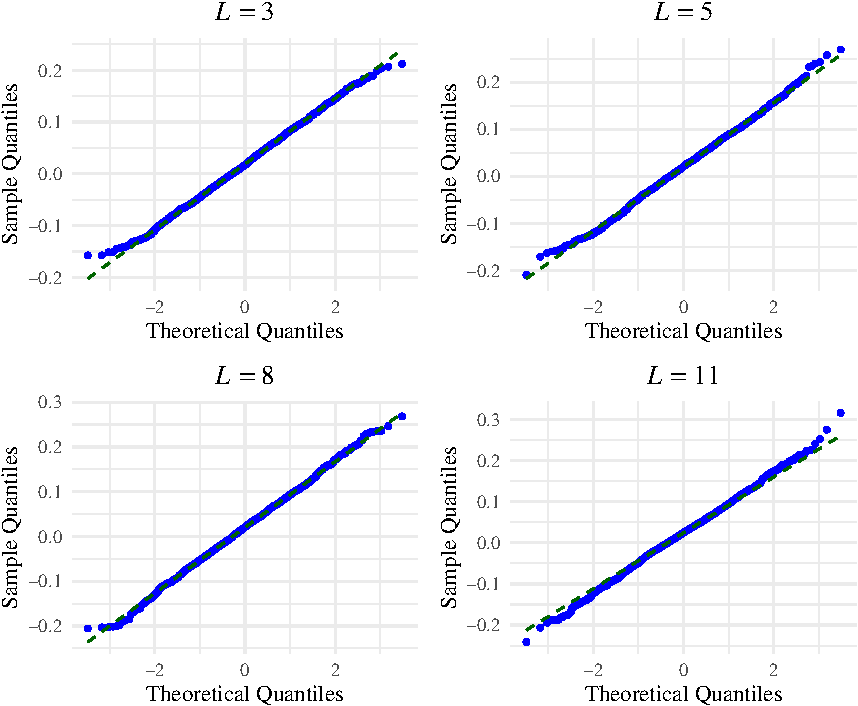
\includegraphics[width=0.8\linewidth]{Identifying-Heterogeneity-in-SAR-Data-with-New-Test-Statistics_files/figure-latex/Plot_normality_qq-1} \caption{Normal QQ-plots for  $n=121$.}\label{fig:Plot_normality_qq}
\end{figure}

After checking the normality of the data, we examined the possibilities of the proposed test in terms of size and power.
Under \(\mathcal{H}_0\), the distribution of the test statistic is asymptotically normal.
Therefore, the \(p\) value is calculated as
\(2\Phi(-\mid \varepsilon\mid)\), where \(\Phi\) is the standard
Gaussian cumulative distribution and \(\varepsilon\) is the standardized test statistic given by :
\[
\varepsilon=\frac{\tilde{H}-H_{\Gamma_{\text{SAR}}}}{\hat\sigma}.
\]

We have nominal levels of \SI{1}{\ percent}, \SI{5}{\ percent}, and
\SI{10}{\percent}. 
In terms of size, \(1000\) simulations were used for different sample sizes with satisfactory results. 
In all cases, the nominal level was achieved. 
The power generally improves with increasing sample size and number of looks.
The results are shown in Table~\ref{tab:table_size_power}.

\hypertarget{the-proposed-test-based-on-coefficient-of-variation-and-a-robust-alternative}{%
\subsection{The Proposed Test Based on Coefficient of Variation and a
Robust
Alternative}\label{the-proposed-test-based-on-coefficient-of-variation-and-a-robust-alternative}}

In addition to the entropy-based test, we also propose a test statistic
based on the classical CV. 
This test statistic is defined as follows:
\begin{align}
    T_{\text{CV}}=\frac{S}{\overline{Z}},
\end{align} 
where \(S\) and \(\overline{Z}\) are the sample standard deviation and the sample mean, respectively.

Similarly, we use another test statistic based on the ratio between the MnAD and the median.
This statistic is given by:
\begin{align}
    T_{\text{CV}_{\text{MnAD}}}=\frac{\text{MnAD}}{\text{Median}}.
\end{align} These test statistics allow assessing the variability of the
data.

The situations in which the use of CV and \(\text{CV}_{\text{MnAD}}\) may be appropriate, i.e.~when the observations are positive, the log-normal
(LN) and the inverse Gaussian distribution (IG) are often more appropriate than the Gamma and Weibull distributions
\cite{Chaubey2017,takagi1997application}.

It is shown that the IG distribution is well approximated by the log-normal distribution, which means that the
IG distribution also does not share the problem of the non-existence of a fixed-width confidence interval with the Gaussian case \cite{whitmore1978}.

The LN distribution in two parameters has the following density
function. 
\begin{align}
    f_Z(z;\mu_{\text{LN}}, \sigma )=\frac{1}{\sigma z\sqrt{2\pi}}\exp\left\{-\frac{(\ln z- \mu_{\text{LN}})^2}{2\sigma^2}\right\}\mathbbm 1_{\mathbbm R_+}(z),
\end{align} here, $\sigma>0$, $-\infty < \mu_{\text{LN}} < \infty$, \(\mu\) is the log-scale parameter and \(\sigma\) is
the shape parameter.

\vskip+1ex
{\color{red} ADCN: Fiz uma diferen\c{c}a entre as nota\c{c}\~oes para m\'edia da G0I e da LN. Por favor, verifique se faz sentido, isto \'e se ela n\~ao \'e encaixada a G0I neste contexto.}
\vskip+1ex

\hypertarget{model-selection-criterion}{%
\subsection{Model Selection Criterion}\label{model-selection-criterion}}

Akaike information criterion (AIC) and Bayesian information criterion
(BIC) are used to select the best fitting distribution.

The AIC is a fine technique that deals with the trade-off between the
goodness-of-fit of the model and the simplicity of the model in terms of
the number of model parameters~\cite{Burnham2004}. The model or
distribution with the lowest value of AIC is chosen to be the best. The
BIC assesses goodness-of-fit of a distribution or model, but avoids
overfitting by penalising an additional degree of
freedom~\cite{Dziak2019}. The model with the lowest BIC value is chosen
as the best.

The AIC and BIC results in
Tables~\ref{tab:table_aic_gamma}-\ref{tab:table_aic_gio_MnADmedian}
indicate that the CV and \(\text{CV}_{\text{MnAD}}\) data from different distributed gamma and \(G_I^0\) synthetic sample sizes match the properties of an LN distribution.
{\color{green}
It is important to note that this conclusion was drawn empirically based on a dictionary of distributions that are anlaytically tractable and well-defined under biparametric, unimodal, asymmetric, and positive distributions.
}
\vskip+1ex
{\color{red} ADCN: 
Caros, esse \'e o ponto mais delicado da excelente ideia desse paper em minha opini\~ao. N\~ao me oponho a colocarmos a lognormal como uma possibilidade, mas \'e preciso deixar claro que \'e uma possibilidade emp\'irica. 
Uma alternativa empirica para uma solu\c{c}\~ao do momento usando distribui\c{c}\~oes mais densenvolvidas na literatura e que sejam analiticamente trat\'aveis. Estou pensando corretamente? Se sim, por que n\~ao log-t-student, log-Laplace, power exponential, Log-hyperbolic,.... (e a lista segue). Sugiro talvez indicar (i) a dedu\c{c}\~ao da distribui\c{c}\~ao assint\'otica das estat\'isticas em fun\c{c}\~ao de CV e MNAD dando com entrada G0I ($\mathcal{H}_1$) e a Gamma ($\mathcal{H}_0$) como trabalho futuro. Do que eu entendi, a suposi\c{c}\~ao da normal assint\'otica para entropia vem de uma cole\c{c}\~ao de trabalhos te\'oricos. 
J\'a a LN, do que percebi, n\~ao.
Coloquei um coment\'ario em verde. Vejam se est\~ao de acordo.
}
\vskip+1ex
The AIC and BIC values of the IG distribution and the LN distribution are not significantly different, as both distributions are based on the right-skewed characteristic. In this situation, the model for the LN distribution was considered the best, as it has the lowest AIC and BIC values.

Figures~\ref{fig:Plot_cv}-\ref{fig:Plot_madmed_gi0_MnADmedian} show empirical and fitted density plots, Q-Q plots, P-P plots as well as empirical and fitted cumulative distribution functions.
They provide qualitative sources that confirm that the LN distribution is the most appropriate distribution.

\begin{table}[H]

\caption{\label{tab:table_aic_gamma}AIC and BIC values for evaluating the best distribution with CV data from Gamma SAR.}
\begin{tabular}[t]{lcccccc}
\toprule
\multicolumn{1}{c}{\textbf{Criterion}} & \multicolumn{1}{c}{$\bm{n}$} & \multicolumn{1}{c}{\textbf{Normal}} & \multicolumn{1}{c}{\textbf{Lognormal}} & \multicolumn{1}{c}{\textbf{Gamma}} & \multicolumn{1}{c}{\textbf{Weibull}} & \multicolumn{1}{c}{\textbf{Inverse Gaussian}}\\
\midrule
 & $25$ & $-38031.95$ & $-38266.75$ & $-38311.84$ & $-36413.23$ & $-38261.60$\\

 & $49$ & $-47698.20$ & $-47913.72$ & $-47905.63$ & $-45553.97$ & $-47911.65$\\

 & $81$ & $-55382.11$ & $-55494.72$ & $-55494.88$ & $-53220.44$ & $-55493.85$\\

\multirow{-4}{*}[1.5\dimexpr\aboverulesep+\belowrulesep+\cmidrulewidth]{\raggedright\arraybackslash AIC} & $121$ & $-61344.92$ & $-61470.83$ & $-61453.83$ & $-58876.04$ & $-61470.48$\\
\cmidrule{1-7}
 & $25$ & $-38016.72$ & $-38251.52$ & $-38296.61$ & $-36397.99$ & $-38246.37$\\

 & $49$ & $-47682.96$ & $-47898.49$ & $-47890.40$ & $-45538.73$ & $-47896.42$\\

 & $81$ & $-55366.88$ & $-55479.49$ & $-55479.65$ & $-53205.21$ & $-55478.62$\\

\multirow{-4}{*}[1.5\dimexpr\aboverulesep+\belowrulesep+\cmidrulewidth]{\raggedright\arraybackslash BIC} & $121$ & $-61329.68$ & $-61455.60$ & $-61438.60$ & $-58860.81$ & $-61455.25$\\
\bottomrule
\end{tabular}
\end{table}

\begin{table}[H]

\caption{\label{tab:table_aic}AIC and BIC values for evaluating the best distribution with CV data from $G_I^0$.}
\begin{tabular}[t]{lcccccc}
\toprule
\multicolumn{1}{c}{\textbf{Criterion}} & \multicolumn{1}{c}{$\bm{n}$} & \multicolumn{1}{c}{\textbf{Normal}} & \multicolumn{1}{c}{\textbf{Lognormal}} & \multicolumn{1}{c}{\textbf{Gamma}} & \multicolumn{1}{c}{\textbf{Weibull}} & \multicolumn{1}{c}{\textbf{Inverse Gaussian}}\\
\midrule
 & $25$ & $\phantom{-}8254.04$ & $\phantom{-}2186.31$ & $\phantom{-}3628.40$ & $\phantom{-}8383.58$ & $\phantom{-}2257.63$\\

 & $49$ & $\phantom{-}8821.79$ & $\phantom{-}1689.03$ & $\phantom{-}3483.10$ & $\phantom{-}9533.53$ & $\phantom{-}1835.29$\\

 & $81$ & $\phantom{-}8525.81$ & $\phantom{-}866.29$ & $\phantom{-}2853.31$ & $\phantom{-}9822.48$ & $\phantom{-}1057.91$\\

\multirow{-4}{*}[1.5\dimexpr\aboverulesep+\belowrulesep+\cmidrulewidth]{\raggedright\arraybackslash AIC} & $121$ & $\phantom{-}8708.81$ & $\phantom{-}131.86$ & $\phantom{-}2341.06$ & $\phantom{-}10506.49$ & $\phantom{-}398.53$\\
\cmidrule{1-7}
 & $25$ & $\phantom{-}8269.27$ & $\phantom{-}2201.54$ & $\phantom{-}3643.63$ & $\phantom{-}8398.81$ & $\phantom{-}2272.86$\\

 & $49$ & $\phantom{-}8837.02$ & $\phantom{-}1704.26$ & $\phantom{-}3498.33$ & $\phantom{-}9548.76$ & $\phantom{-}1850.52$\\

 & $81$ & $\phantom{-}8541.04$ & $\phantom{-}881.52$ & $\phantom{-}2868.55$ & $\phantom{-}9837.72$ & $\phantom{-}1073.14$\\

\multirow{-4}{*}[1.5\dimexpr\aboverulesep+\belowrulesep+\cmidrulewidth]{\raggedright\arraybackslash BIC} & $121$ & $\phantom{-}8724.04$ & $\phantom{-}147.09$ & $\phantom{-}2356.29$ & $\phantom{-}10521.72$ & $\phantom{-}413.76$\\
\bottomrule
\end{tabular}
\end{table}

\begin{table}[H]

\caption{\label{tab:table_aic_gamma_madmed}AIC and BIC values for evaluating the best distribution with $\text{CV}_{\text{MnAD}}$ data from Gamma SAR.}
\begin{tabular}[t]{lcccccc}
\toprule
\multicolumn{1}{c}{\textbf{Criterion}} & \multicolumn{1}{c}{$\bm{n}$} & \multicolumn{1}{c}{\textbf{Normal}} & \multicolumn{1}{c}{\textbf{Lognormal}} & \multicolumn{1}{c}{\textbf{Gamma}} & \multicolumn{1}{c}{\textbf{Weibull}} & \multicolumn{1}{c}{\textbf{Inverse Gaussian}}\\
\midrule
 & $25$ & $-38375.56$ & $-39147.85$ & $-39066.29$ & $-36652.49$ & $-39143.61$\\

 & $49$ & $-48386.11$ & $-48795.32$ & $-48745.48$ & $-46240.91$ & $-48793.83$\\

 & $81$ & $-56072.87$ & $-56322.32$ & $-56290.02$ & $-53836.04$ & $-56322.12$\\

\multirow{-4}{*}[1.5\dimexpr\aboverulesep+\belowrulesep+\cmidrulewidth]{\raggedright\arraybackslash AIC} & $121$ & $-62217.14$ & $-62394.77$ & $-62369.32$ & $-59861.80$ & $-62394.57$\\
\cmidrule{1-7}
 & $25$ & $-38360.32$ & $-39132.62$ & $-39051.05$ & $-36637.26$ & $-39128.38$\\

 & $49$ & $-48370.87$ & $-48780.09$ & $-48730.25$ & $-46225.67$ & $-48778.60$\\

 & $81$ & $-56057.64$ & $-56307.09$ & $-56274.79$ & $-53820.81$ & $-56306.89$\\

\multirow{-4}{*}[1.5\dimexpr\aboverulesep+\belowrulesep+\cmidrulewidth]{\raggedright\arraybackslash BIC} & $121$ & $-62201.91$ & $-62379.54$ & $-62354.09$ & $-59846.56$ & $-62379.33$\\
\bottomrule
\end{tabular}
\end{table}

\begin{table}[H]

\caption{\label{tab:table_aic_gio_MnADmedian}AIC and BIC values for evaluating the best distribution with $\text{CV}_{\text{MnAD}}$ data from $G_I^0$.}
\begin{tabular}[t]{lcccccc}
\toprule
\multicolumn{1}{c}{\textbf{Criterion}} & \multicolumn{1}{c}{$\bm{n}$} & \multicolumn{1}{c}{\textbf{Normal}} & \multicolumn{1}{c}{\textbf{Lognormal}} & \multicolumn{1}{c}{\textbf{Gamma}} & \multicolumn{1}{c}{\textbf{Weibull}} & \multicolumn{1}{c}{\textbf{Inverse Gaussian}}\\
\midrule
 & $25$ & $-13302.39$ & $-15575.23$ & $-15158.42$ & $-11933.35$ & $-15565.03$\\

 & $49$ & $-23265.27$ & $-24529.72$ & $-24284.47$ & $-20986.94$ & $-24522.28$\\

 & $81$ & $-29908.19$ & $-30960.38$ & $-30747.90$ & $-25233.41$ & $-30946.54$\\

\multirow{-4}{*}[1.5\dimexpr\aboverulesep+\belowrulesep+\cmidrulewidth]{\raggedright\arraybackslash AIC} & $121$ & $-36496.78$ & $-37128.07$ & $-36991.41$ & $-32366.52$ & $-37123.20$\\
\cmidrule{1-7}
 & $25$ & $-13287.16$ & $-15559.99$ & $-15143.19$ & $-11918.12$ & $-15549.80$\\

 & $49$ & $-23250.04$ & $-24514.48$ & $-24269.24$ & $-20971.71$ & $-24507.05$\\

 & $81$ & $-29892.96$ & $-30945.15$ & $-30732.67$ & $-25218.17$ & $-30931.31$\\

\multirow{-4}{*}[1.5\dimexpr\aboverulesep+\belowrulesep+\cmidrulewidth]{\raggedright\arraybackslash BIC} & $121$ & $-36481.55$ & $-37112.84$ & $-36976.18$ & $-32351.28$ & $-37107.97$\\
\bottomrule
\end{tabular}
\end{table}

\begin{figure}[H]

{\centering 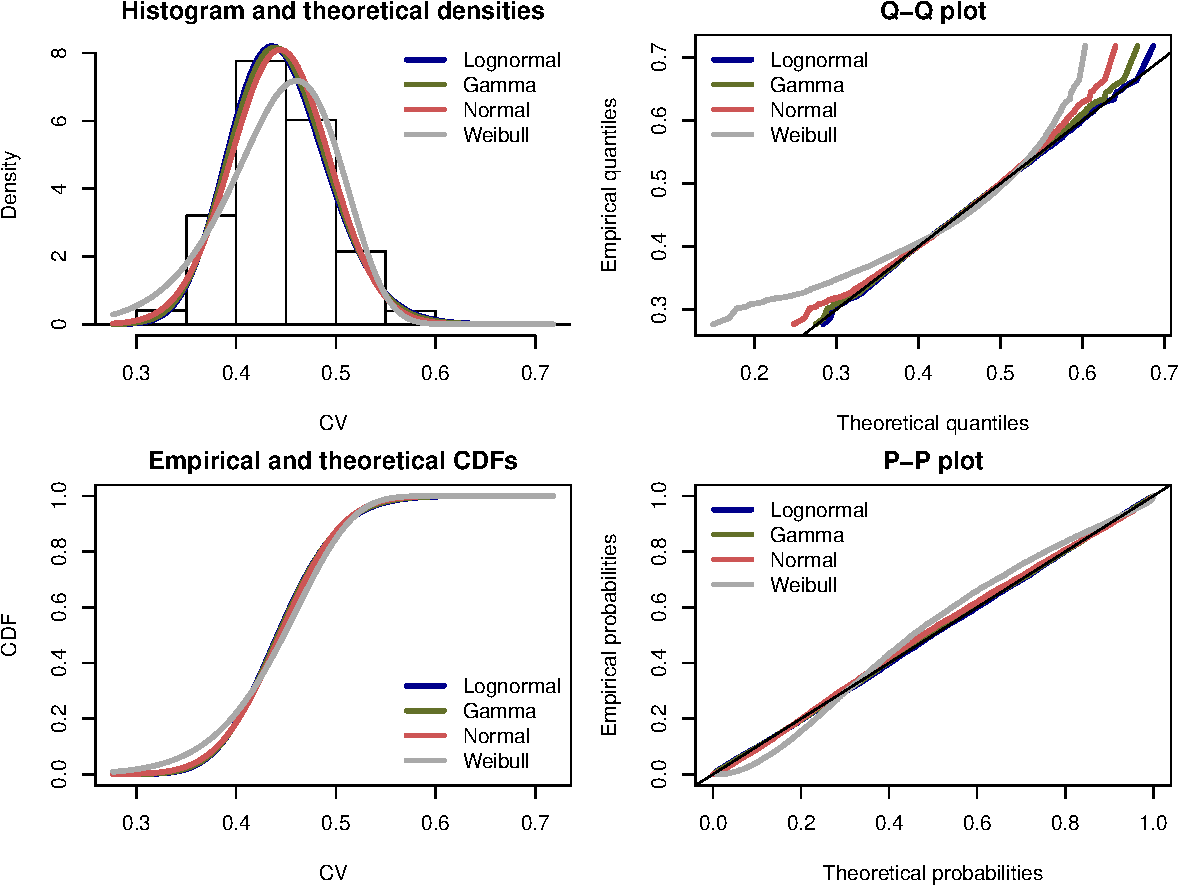
\includegraphics[width=1\linewidth]{Identifying-Heterogeneity-in-SAR-Data-with-New-Test-Statistics_files/figure-latex/Plot_cv_gamma-1} 

}

\caption{Goodness of fit plots for evaluating the best distribution with CV data from Gamma SAR, with  $n=49$, $L=5$ and $\mu=1$.}\label{fig:Plot_cv_gamma}
\end{figure}

\begin{figure}[H]

{\centering 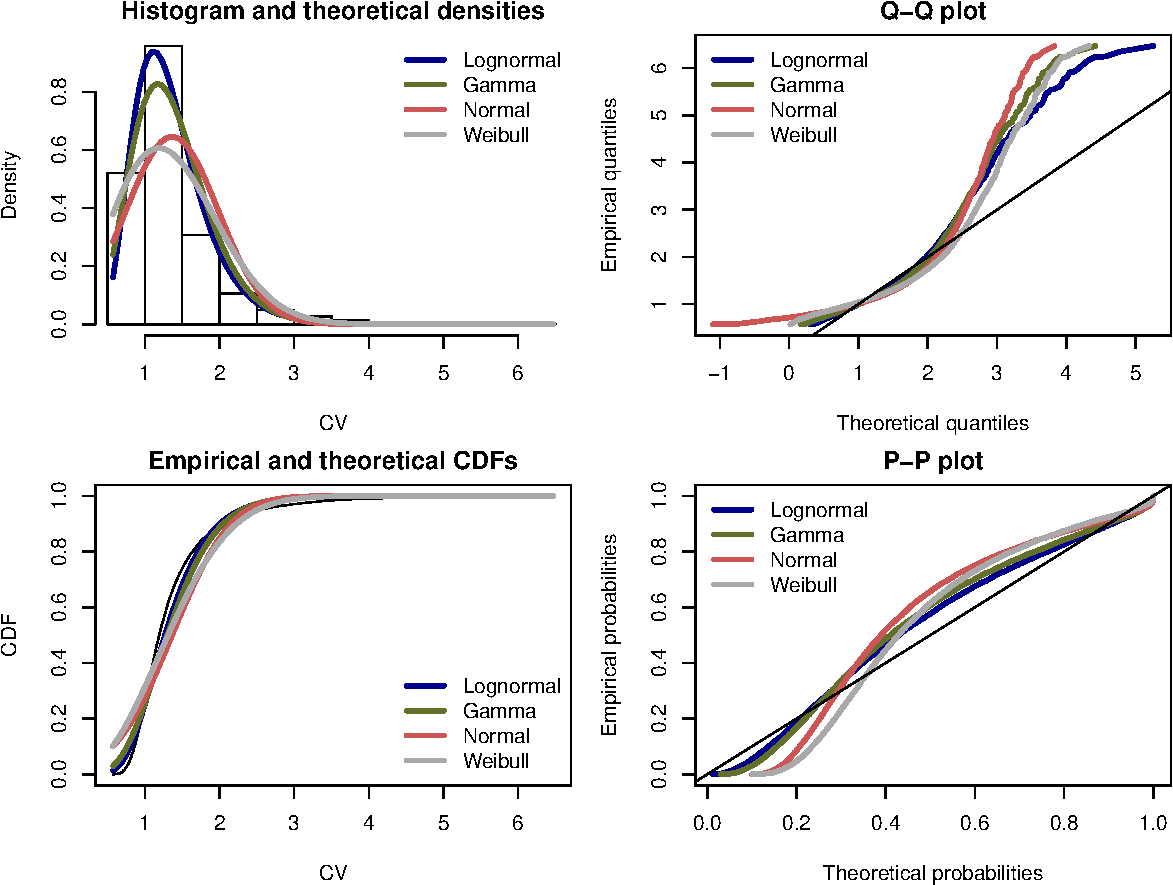
\includegraphics[width=1\linewidth]{Identifying-Heterogeneity-in-SAR-Data-with-New-Test-Statistics_files/figure-latex/Plot_cv-1} 

}

\caption{Goodness of fit plots for evaluating the best distribution with $\text{CV}_{\text{MnAD}}$ data from $G_I^0$, with  $n=49$, $L=5$, $\mu=1$ and $\alpha=-2$.}\label{fig:Plot_cv}
\end{figure}

\begin{figure}[H]

{\centering 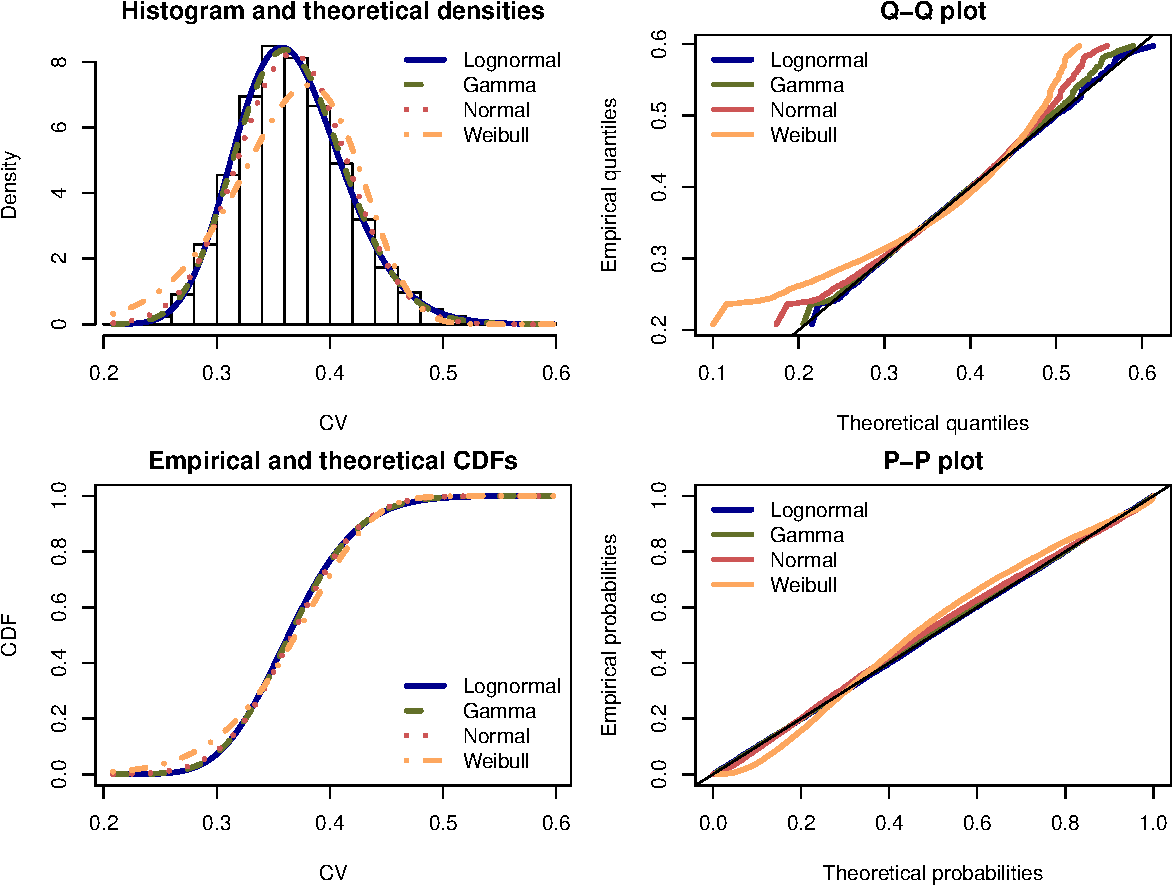
\includegraphics[width=1\linewidth]{Identifying-Heterogeneity-in-SAR-Data-with-New-Test-Statistics_files/figure-latex/Plot_MnADmedian_gamma-1} 

}

\caption{Goodness of fit plots for evaluating the best distribution with $\text{CV}_{\text{MnAD}}$ data from Gamma SAR, with  $n=49$, $L=5$ and $\mu=1$.}\label{fig:Plot_MnADmedian_gamma}
\end{figure}

\begin{figure}[hbt]
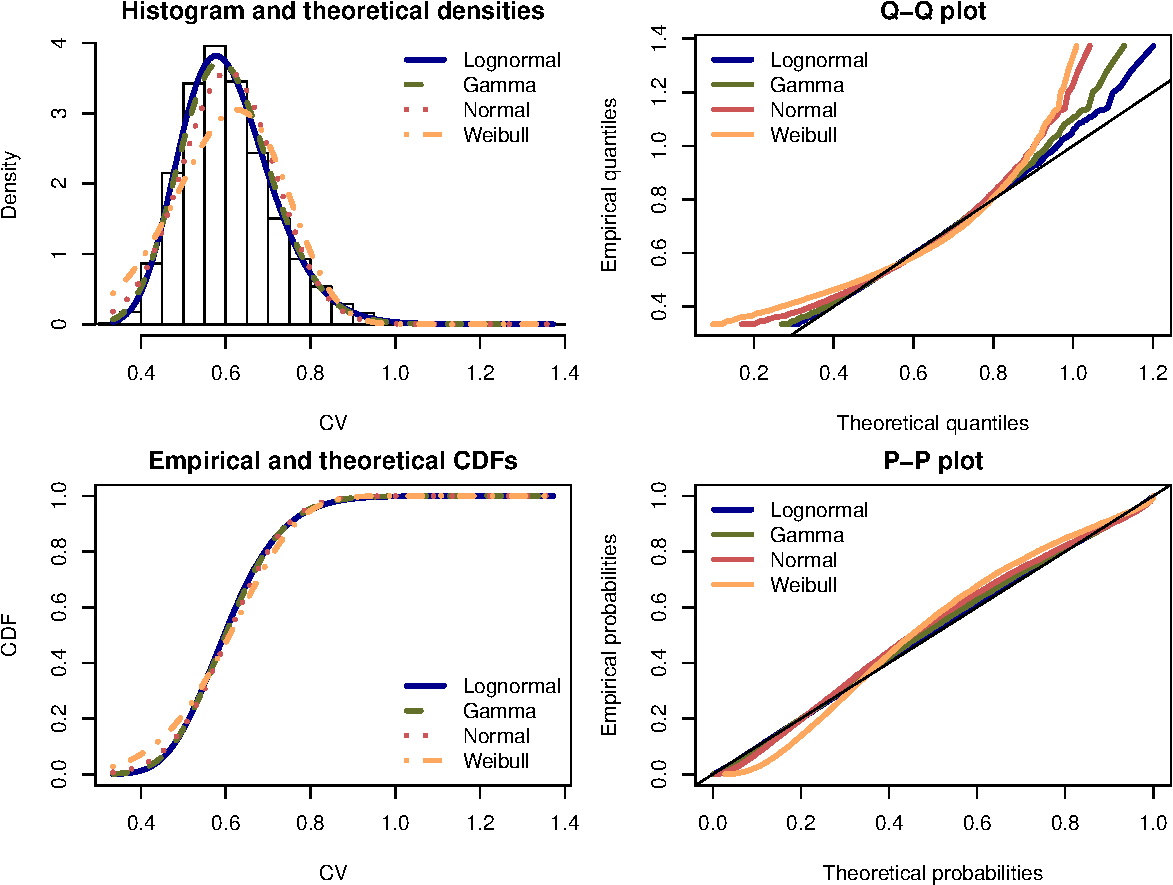
\includegraphics[width=1\linewidth]{Identifying-Heterogeneity-in-SAR-Data-with-New-Test-Statistics_files/figure-latex/Plot_madmed_gi0_MnADmedian-1} \caption{Goodness of fit plots for evaluating the best distribution with $CV_{\text{MnAD}}$ data from $G_I^0$, with  $n=49$, $L=5$, $\mu=1$ and $\alpha=-5$.}\label{fig:Plot_madmed_gi0_MnADmedian}
\end{figure}

\hypertarget{sec:Results}{%
\section{Simulation Results}\label{sec:Results}}

This section presents simulations that were performed to obtain an evaluation of the performance of the proposed test statistics.

\hypertarget{simulated-data}{%
\subsection{Simulated Data}\label{simulated-data}}

Figure~\ref{fig:sim_SAR_Images}(a) shows the phantom used for a simulated image with dimensions of \(250\times 250\) pixels to show the differences between heterogeneous (dark, \(\alpha=-2\))
and homogeneous (light, \(\alpha=-10\)) regions, with \(L = 5\). 
The regions are formed by independent draws from the \(G^0_I\) distribution.

The three test statistics are applied to the simulated image using local
sliding windows of size \(7\times 7\).

The resulting \(p\)-values for the tests \(S_H\), \(T_{\text{CV}}\), and
\(T_{\text{CV}_{\text{MnAD}}}\) are shown in
Figures~\ref{fig:sim_SAR_Images}(b)-(d) and
Figures~\ref{fig:sim_SAR_Images_p05}(a)-(c), respectively. 
The new images reveal that a darker background indicates homogeneity, while lighter backgrounds represent heterogeneous areas.

\begin{figure}[H]

{\centering \subfloat[\label{fig:sim_SAR_Images-1}]{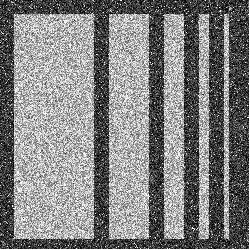
\includegraphics[width=40mm]{../Figures/PNG/simulated7x7} }\subfloat[\label{fig:sim_SAR_Images-2}]{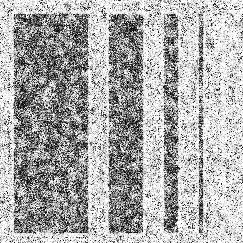
\includegraphics[width=40mm]{../Figures/PNG/sim_pvalue7x7_total_H} }\subfloat[\label{fig:sim_SAR_Images-3}]{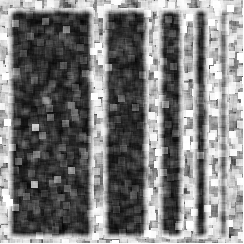
\includegraphics[width=40mm]{../Figures/PNG/sim_pvalue7x7_total_cv} }\newline\subfloat[\label{fig:sim_SAR_Images-4}]{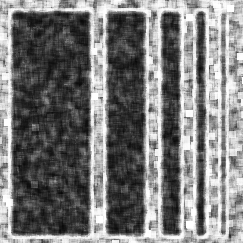
\includegraphics[width=40mm]{../Figures/PNG/sim_pvalue7x7_total_mnad} }

}

\caption{Results of applying the test statistics. (a) Simulated image; $P$-values from the entropy-based test; (c) $P$-values from the CV test; (d) $P$-values from the   $\text{CV}_{\text{MnAD}}$ test; }\label{fig:sim_SAR_Images}
\end{figure}
\begin{figure}[H]

{\centering \subfloat[ \label{fig:sim_SAR_Images_p05-1}]{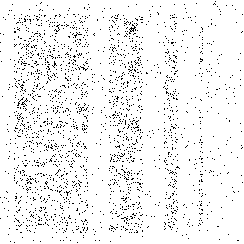
\includegraphics[width=40mm]{../Figures/PNG/sim_pvalue7x7_H} }\subfloat[ \label{fig:sim_SAR_Images_p05-2}]{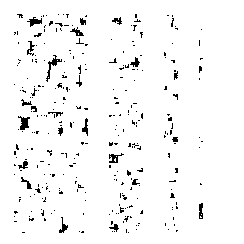
\includegraphics[width=40mm]{../Figures/PNG/sim_pvalue7x7_cv} }\subfloat[ \label{fig:sim_SAR_Images_p05-3}]{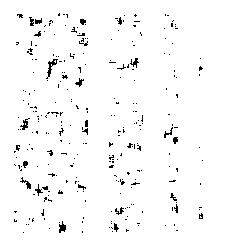
\includegraphics[width=40mm]{../Figures/PNG/sim_pvalue7x7_mnad} }

}

\caption{Results of tests on simulated data with a threshold of $0.1$ of the $p$-value. (a) Entropy-based test; (b) CV test; (c) $\text{CV}_{\text{MnAD}}$ test.}\label{fig:sim_SAR_Images_p05}
\end{figure}

\hypertarget{real-data}{%
\subsection{Real Data}\label{real-data}}

We evaluated the proposed test statistic using two real SAR images. 
For our analysis, we used images of the city of Frankfurt, Germany, and of
Ottawa, Canada. 
These images were acquired by the Sentinel-1A satellite operating in C-band, with VV polarization, intensity format and
\(L=5\) nominal looks.
Both images have a size of \(512 \times 512\) pixels and contain urban areas, water and forest regions, as shown in
Figures~\ref{fig:real_SAR_Images_coe}(a)-(b).

The \(p\)-values obtained for the \(S_H\), \(T_{\text{CV}}\), and
\(T_{\text{CV}_{\text{MnAD}}}\) tests are presented in
Figures~\ref{fig:sim_SAR_Images_Frankfurt}-\ref{fig:sim_SAR_Images_01_Ottawa},
respectively.

In general, using the original and robust CV is more meaningful than using Shannon entropy to capture texturelessness.
It is justified that the dark areas of the maps based on the $\text{CV}$ and $\text{CV}_{\text{MnAD}}$ tests cover the areas reported for the Shannon entropy-based map.
Both CV-based tools predicted textureless regions as well as boundaries where the statistical properties of texture vary.
Assuming $10\%$ as the threshold for the $p$ values, the dark region produced by the $\text{CV}$ test was higher than that produced by the $\text{CV}_{\text{MnAD}}$ and entropy test.
The latter observation is to be expected as the latter tests are robust alternatives to the former test, which is essentially based on the expected value operator that reacts to outliers.


\begin{figure}[H]

{\centering \subfloat[ \label{fig:real_SAR_Images_coe-1}]{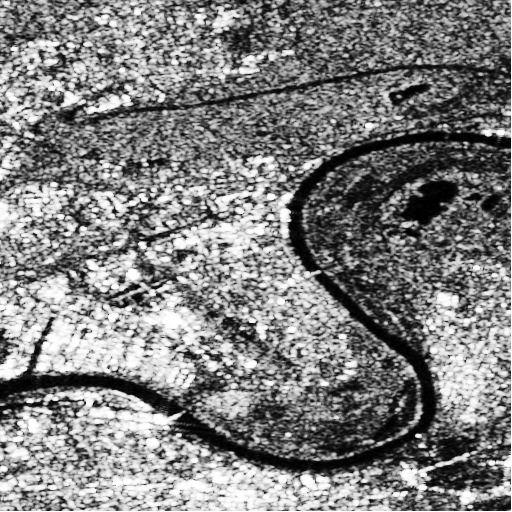
\includegraphics[width=40mm]{../Figures/PNG/Intensity_Frankfurt_512_n} }\subfloat[ \label{fig:real_SAR_Images_coe-2}]{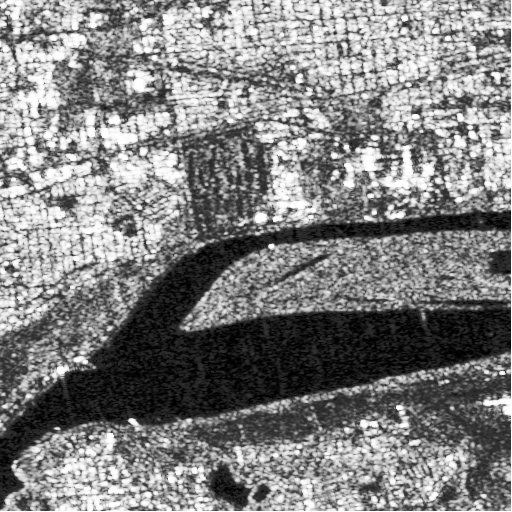
\includegraphics[width=40mm]{../Figures/PNG/Intensity_Ottawa_512_n} }

}

\caption{SAR images. (a) Frankfurt; (b) Ottawa. }\label{fig:real_SAR_Images_coe}
\end{figure}
\begin{figure}[H]

{\centering \subfloat[ \label{fig:sim_SAR_Images_Frankfurt-1}]{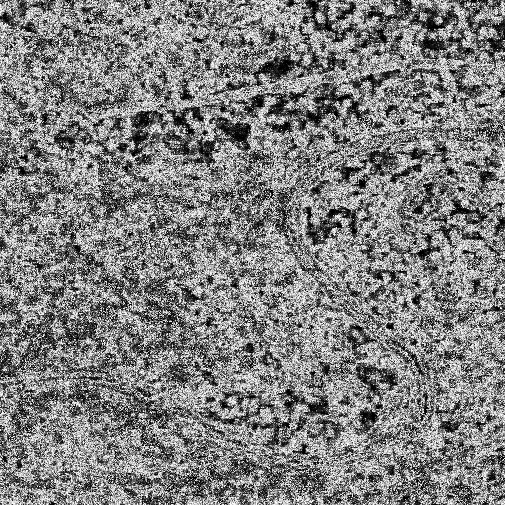
\includegraphics[width=40mm]{../Figures/PNG/Frankfurt_512_pvalue7x7_total_H} }\subfloat[ \label{fig:sim_SAR_Images_Frankfurt-2}]{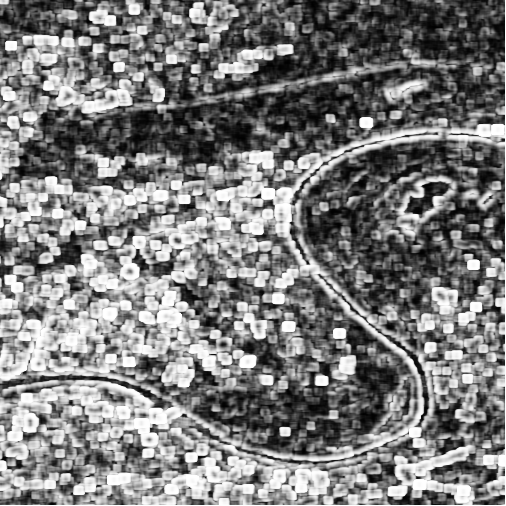
\includegraphics[width=40mm]{../Figures/PNG/Frankfurt_512_pvalue7x7_total_CV} }\subfloat[ \label{fig:sim_SAR_Images_Frankfurt-3}]{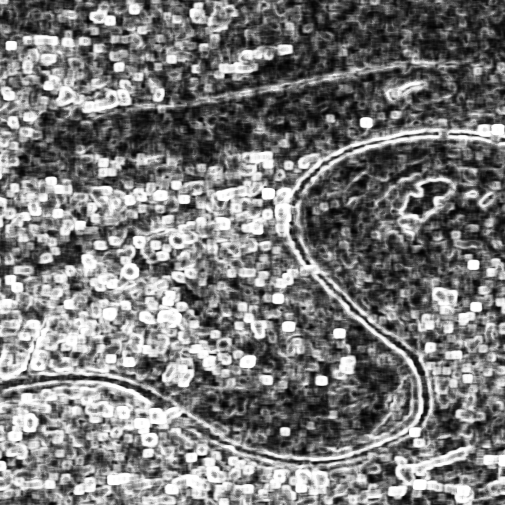
\includegraphics[width=40mm]{../Figures/PNG/Frankfurt_512_mnad_7_total} }

}

\caption{Results of applying the test statistics in Frankfurt image. (a) $P$-values from the entropy-based test; (b) $P$-values from the CV test; (c) $P$-values from the   $\text{CV}_{\text{MnAD}}$ test. }\label{fig:sim_SAR_Images_Frankfurt}
\end{figure}
\begin{figure}[H]

{\centering \subfloat[ \label{fig:sim_SAR_Images_01Frankfurt-1}]{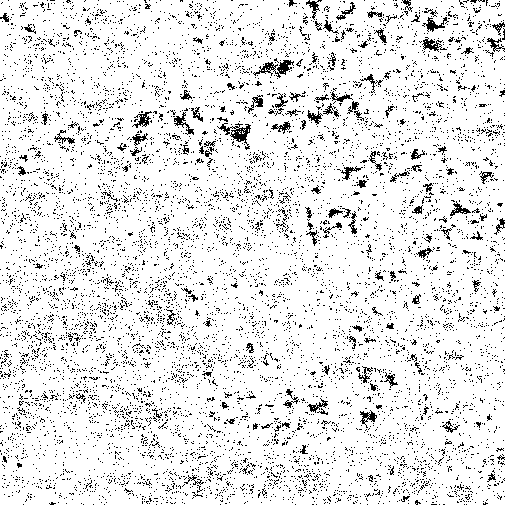
\includegraphics[width=40mm]{../Figures/PNG/Frankfurt_512_pvalue7x7_H_01} }\subfloat[ \label{fig:sim_SAR_Images_01Frankfurt-2}]{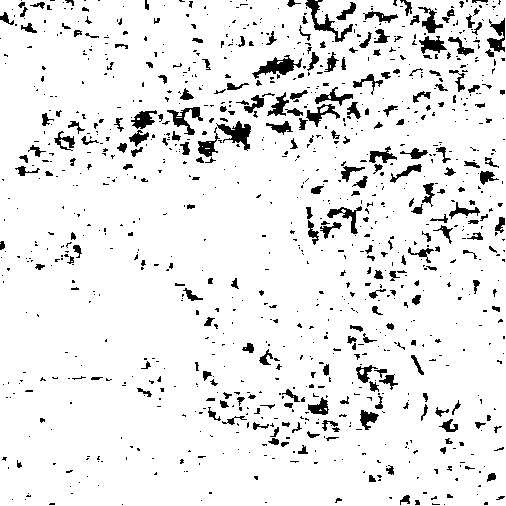
\includegraphics[width=40mm]{../Figures/PNG/Frankfurt_512_pvalue7x7_CV} }\subfloat[ \label{fig:sim_SAR_Images_01Frankfurt-3}]{
\includegraphics[width=40mm]{../Figures/PNG/Frankfurt_512_mnad_7_0.1} }

}

\caption{Test results with a threshold of $0.1$ of the $p$-value for the Frankfurt image. (a) Entropy-based test; (b) CV test; (c) $\text{CV}_{\text{MnAD}}$ test.}\label{fig:sim_SAR_Images_01Frankfurt}
\end{figure}

\begin{figure}[H]

{\centering \subfloat[ \label{fig:sim_SAR_Images_Ottawa-1}]{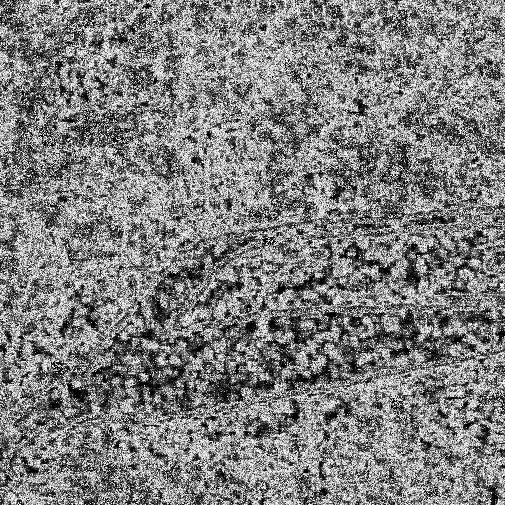
\includegraphics[width=40mm]{../Figures/PNG/Ottawa_512_pvalue7x7_total_H} }\subfloat[ \label{fig:sim_SAR_Images_Ottawa-2}]{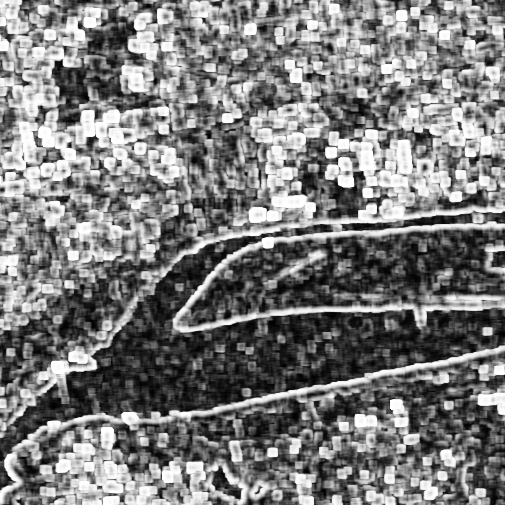
\includegraphics[width=40mm]{../Figures/PNG/Ottawa_512_CV_pvalue7x7_total_CV} }\subfloat[ \label{fig:sim_SAR_Images_Ottawa-3}]{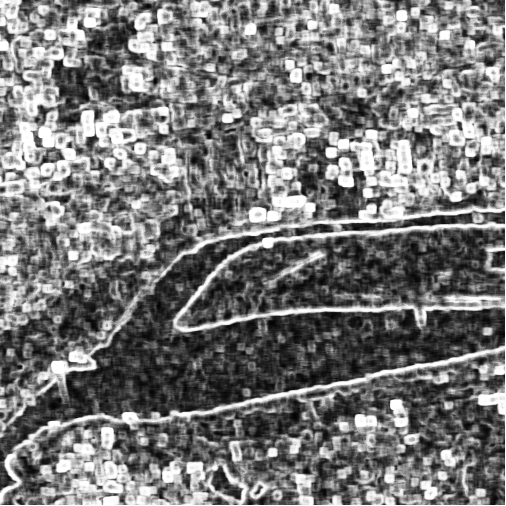
\includegraphics[width=40mm]{../Figures/PNG/Ottawa_512_mnad_7_total} }

}

\caption{Results of applying the test statistics in Ottawa image. (a) $P$-values from the entropy-based test; (b) $P$-values from the CV test; (c) $P$-values from the   $\text{CV}_{\text{MnAD}}$ test.}\label{fig:sim_SAR_Images_Ottawa}
\end{figure}
\begin{figure}[H]

{\centering \subfloat[ \label{fig:sim_SAR_Images_01_Ottawa-1}]{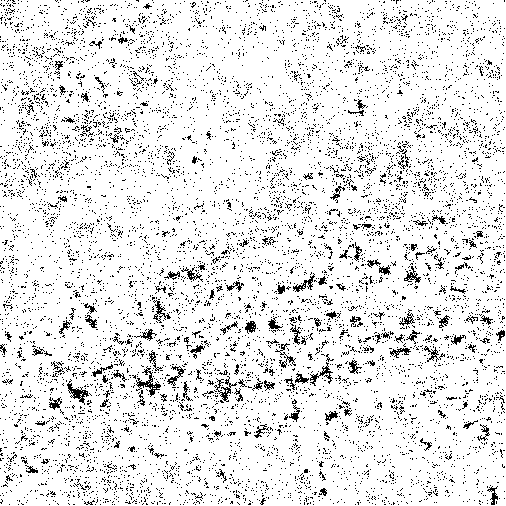
\includegraphics[width=40mm]{../Figures/PNG/Ottawa_512_pvalue7x7_H_01} }\subfloat[ \label{fig:sim_SAR_Images_01_Ottawa-2}]{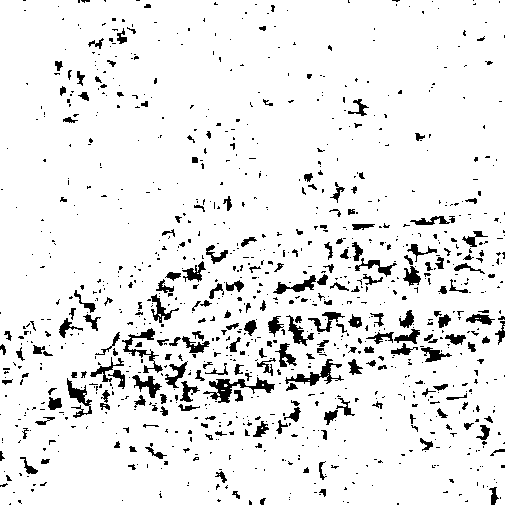
\includegraphics[width=40mm]{../Figures/PNG/Ottawa_512_CV_pvalue7x7_CV} }\subfloat[ \label{fig:sim_SAR_Images_01_Ottawa-3}]{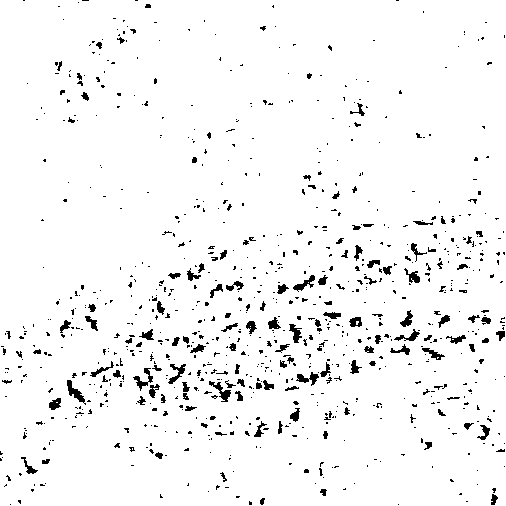
\includegraphics[width=40mm]{../Figures/PNG/Ottawa_512_mnad_7_0.1} }

}

\caption{Test results with a threshold of $0.1$ of the $p$-value for the Ottawa image. (a) Entropy-based test; (b) CV test; (c) $\text{CV}_{\text{MnAD}}$ test.}\label{fig:sim_SAR_Images_01_Ottawa}
\end{figure}

\hypertarget{sec:conclusion}{%
\section{Conclusion}\label{sec:conclusion}}

In this article, we have provided a practical and theoretical answer to the following physical question: How to detect texturelessness in SAR images, assuming that the SAR intensity follows the $\mathcal{G}^0_I$ distribution.
Solving this problem is not easy, considering that the texturelessness in the parametric space of $\mathcal{G}^0_I$ means the infinity value, which is neither analitically tractable nor practically provable.
To this end, we proposed three novel hypothesis tests, one from the Shannon entropy and two others from the variation coefficient variants.
The performance of our proposals was evaluated using a Monte Carlo study. The results showed that they were conservative in estimating the probability of a type I error (false alarm rate) and the test power (probability of detection), which increases with sample size.
An application to two recent SAR images was performed. The results showed that the $\text{CV}_{\text{MnAD}}$ and Shannon entropy-based tests were more robust than the CV-based tests. In addition, the CV-based tests were able to recognize both images without texture and those where the type of texture changes.


%%%%%%%%%%%%%%%%%%%%%%%%%%%%%%%%%%%%%%%%%%

\vspace{6pt}

%%%%%%%%%%%%%%%%%%%%%%%%%%%%%%%%%%%%%%%%%%
%% optional
\supplementary{This article is fully reproducible using RMarkdown. All
code and data are accessible at
\url{https://github.com/rjaneth/identifying-heterogeneity-in-sar-data-with-new-test-statistics}
(accessed on 5 April 2024).}

% Only for the journal Methods and Protocols:
% If you wish to submit a video article, please do so with any other supplementary material.
% \supplementary{The following supporting information can be downloaded at: \linksupplementary{s1}, Figure S1: title; Table S1: title; Video S1: title. A supporting video article is available at doi: link.}

%%%%%%%%%%%%%%%%%%%%%%%%%%%%%%%%%%%%%%%%%%
\authorcontributions{For research articles with several authors, a short
paragraph specifying their individual contributions must be provided.
The following statements should be used ``X.X. and Y.Y. conceive and
designed the experiments; X.X. performed the experiments; X.X. and Y.Y.
analyzed the data; W.W. contributed reagents/materials/analysis tools;
Y.Y. wrote the paper.'\,' Authorship must be limited to those who have
contributed substantially to the work reported.}

\funding{Please add: ``This research received no external funding'' or
``This research was funded by NAME OF FUNDER grant number XXX.'' and
``The APC was funded by XXX'\,'. Check carefully that the details given
are accurate and use the standard spelling of funding agency names at
\url{https://search.crossref.org/funding}, any errors may affect your
future funding.}

\institutionalreview{Not applicable.}


\dataavailability{Not applicable.}

\acknowledgments{This study was financed in part by the Coordenação de
Aperfeiçoamento de Pessoal de Nível Superior - Brasil (CAPES) - Finance
Code 001.}

\conflictsofinterest{The authors declare no conflict of interest.}

%%%%%%%%%%%%%%%%%%%%%%%%%%%%%%%%%%%%%%%%%%
%% Optional

%% Only for journal Encyclopedia


%%%%%%%%%%%%%%%%%%%%%%%%%%%%%%%%%%%%%%%%%%
%% Optional
%%%%%%%%%%%%%%%%%%%%%%%%%%%%%%%%%%%%%%%%%%
\begin{adjustwidth}{-\extralength}{0cm}

%\printendnotes[custom] % Un-comment to print a list of endnotes


\reftitle{References}
\bibliography{references.bib}

% If authors have biography, please use the format below
%\section*{Short Biography of Authors}
%\bio
%{\raisebox{-0.35cm}{\includegraphics[width=3.5cm,height=5.3cm,clip,keepaspectratio]{Definitions/author1.pdf}}}
%{\textbf{Firstname Lastname} Biography of first author}
%
%\bio
%{\raisebox{-0.35cm}{\includegraphics[width=3.5cm,height=5.3cm,clip,keepaspectratio]{Definitions/author2.jpg}}}
%{\textbf{Firstname Lastname} Biography of second author}

%%%%%%%%%%%%%%%%%%%%%%%%%%%%%%%%%%%%%%%%%%
%% for journal Sci
%\reviewreports{\\
%Reviewer 1 comments and authors’ response\\
%Reviewer 2 comments and authors’ response\\
%Reviewer 3 comments and authors’ response
%}
%%%%%%%%%%%%%%%%%%%%%%%%%%%%%%%%%%%%%%%%%%
\PublishersNote{}
\end{adjustwidth}


\end{document}
